\section{Introduction}


%%%%%%%%%%%%%%%%%%%%%%%%%%%%%%%%%%%%%%%%%%%%%%%%%%%%%%%%%%%%%%%%%%%%%%%%%%%%%%%
\section{Methodology}

We start with Euler's homogeneity equation \citep{Thompson1982,Reid1990}

\begin{equation}
  (x - x_o)\partial_x f + (y - y_o)\partial_y f + (z - z_o)\partial_z f
  + \eta(f - b)
  \ ,
  \label{eq:euler}
\end{equation}

\noindent
in which $f$ is a homogeneous function (in this case, a potential-field),
$(x, y, z)$ are the coordinates of the observation point,
$(x_o, y_o, z_o)$ are the coordinates of the field source,
$b$ is the base level representing a constant shift in the field,
and $\eta$ is the structural index, which is related to the nature of the
source and how its potential-field values decay with distance.
Starting with \citet{Thompson1982} and \citet{Reid1990}, Euler's equation has
been used to estimate the source positions of gravity and magnetic data.
In this section, we will review the solution of Equation~\ref{eq:euler} for
$(x_o, y_o, z_o)$ by Euler Deconvolution and then present a new method, called
Euler Inversion, for solving Euler's equation using total least-squares.

\subsection{Euler deconvolution}


\subsection{Euler inversion}


Starting values for p and d.

\subsection{Estimating the structural index}

\subsection{Windowing procedure}


%%%%%%%%%%%%%%%%%%%%%%%%%%%%%%%%%%%%%%%%%%%%%%%%%%%%%%%%%%%%%%%%%%%%%%%%%%%%%%%
\section{Results}


\subsection{Method demonstration with a single window}

\begin{figure}[tb!]
\centering
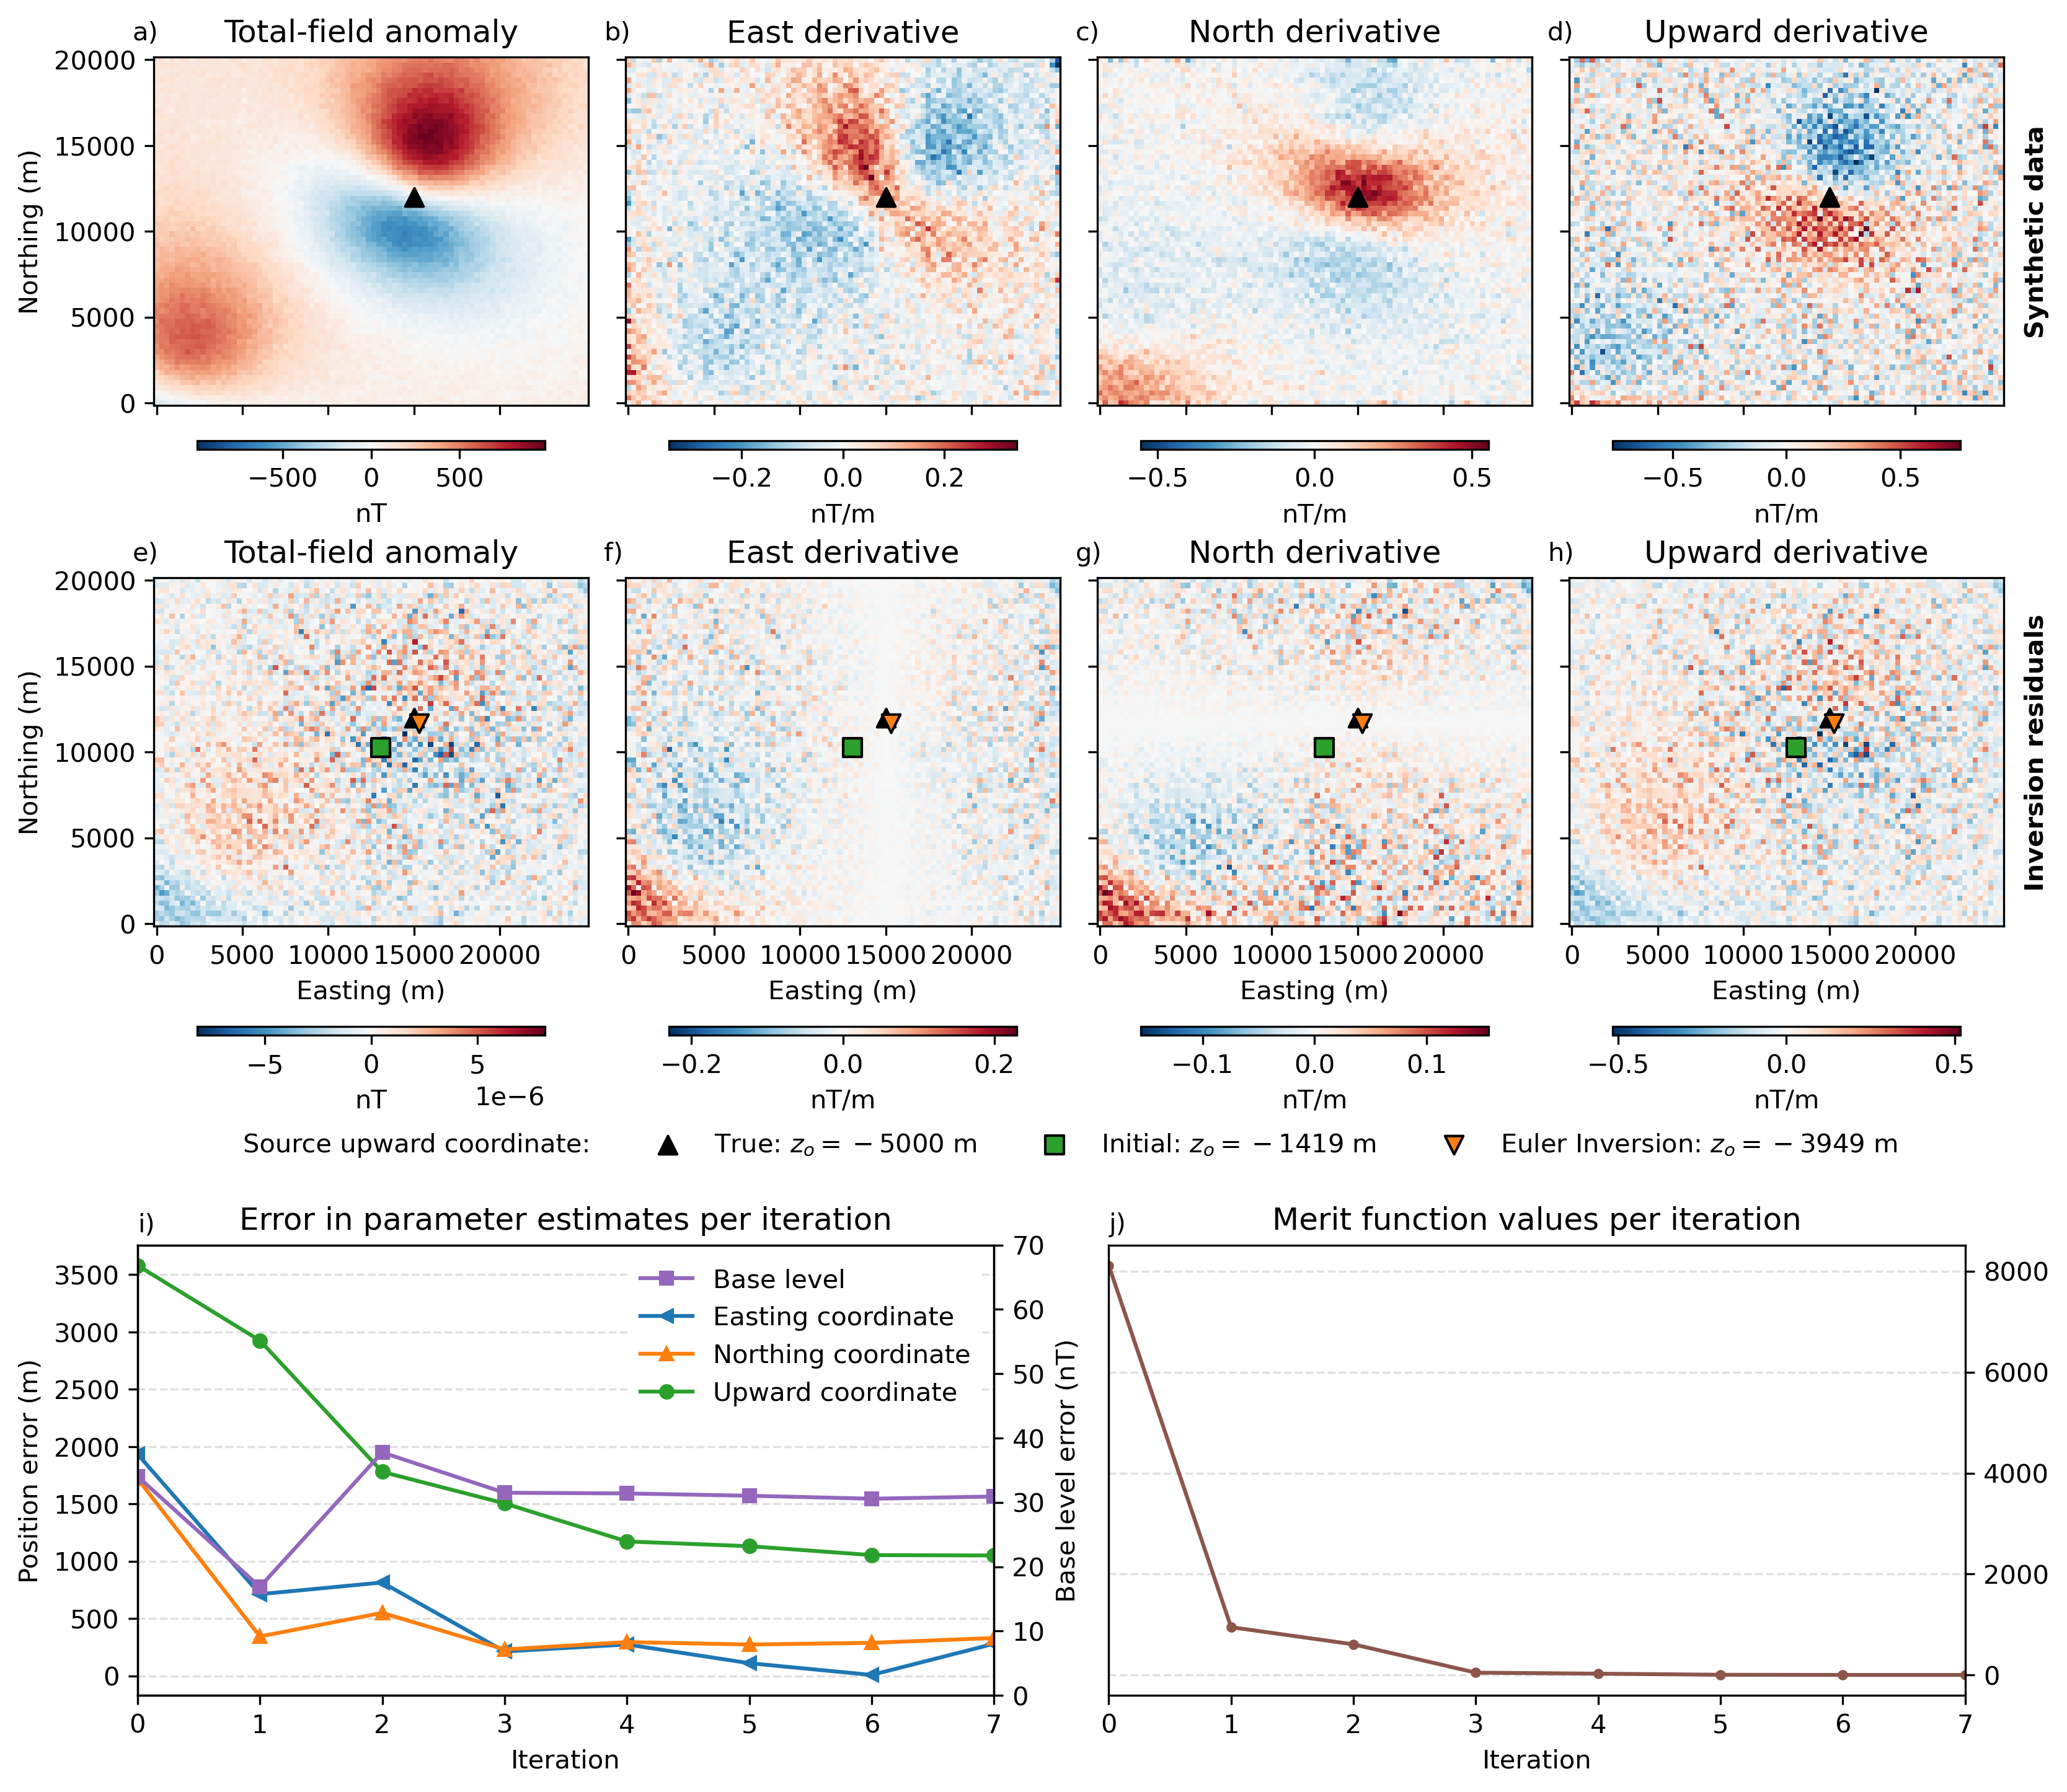
\includegraphics[width=1\linewidth]{figures/synthetic-proof-of-concept.png}
\caption{
  \lipsum[1]
}
\label{fig:proof}
\end{figure}


\subsection{Effect of random noise}

\begin{figure}[tb!]
\centering
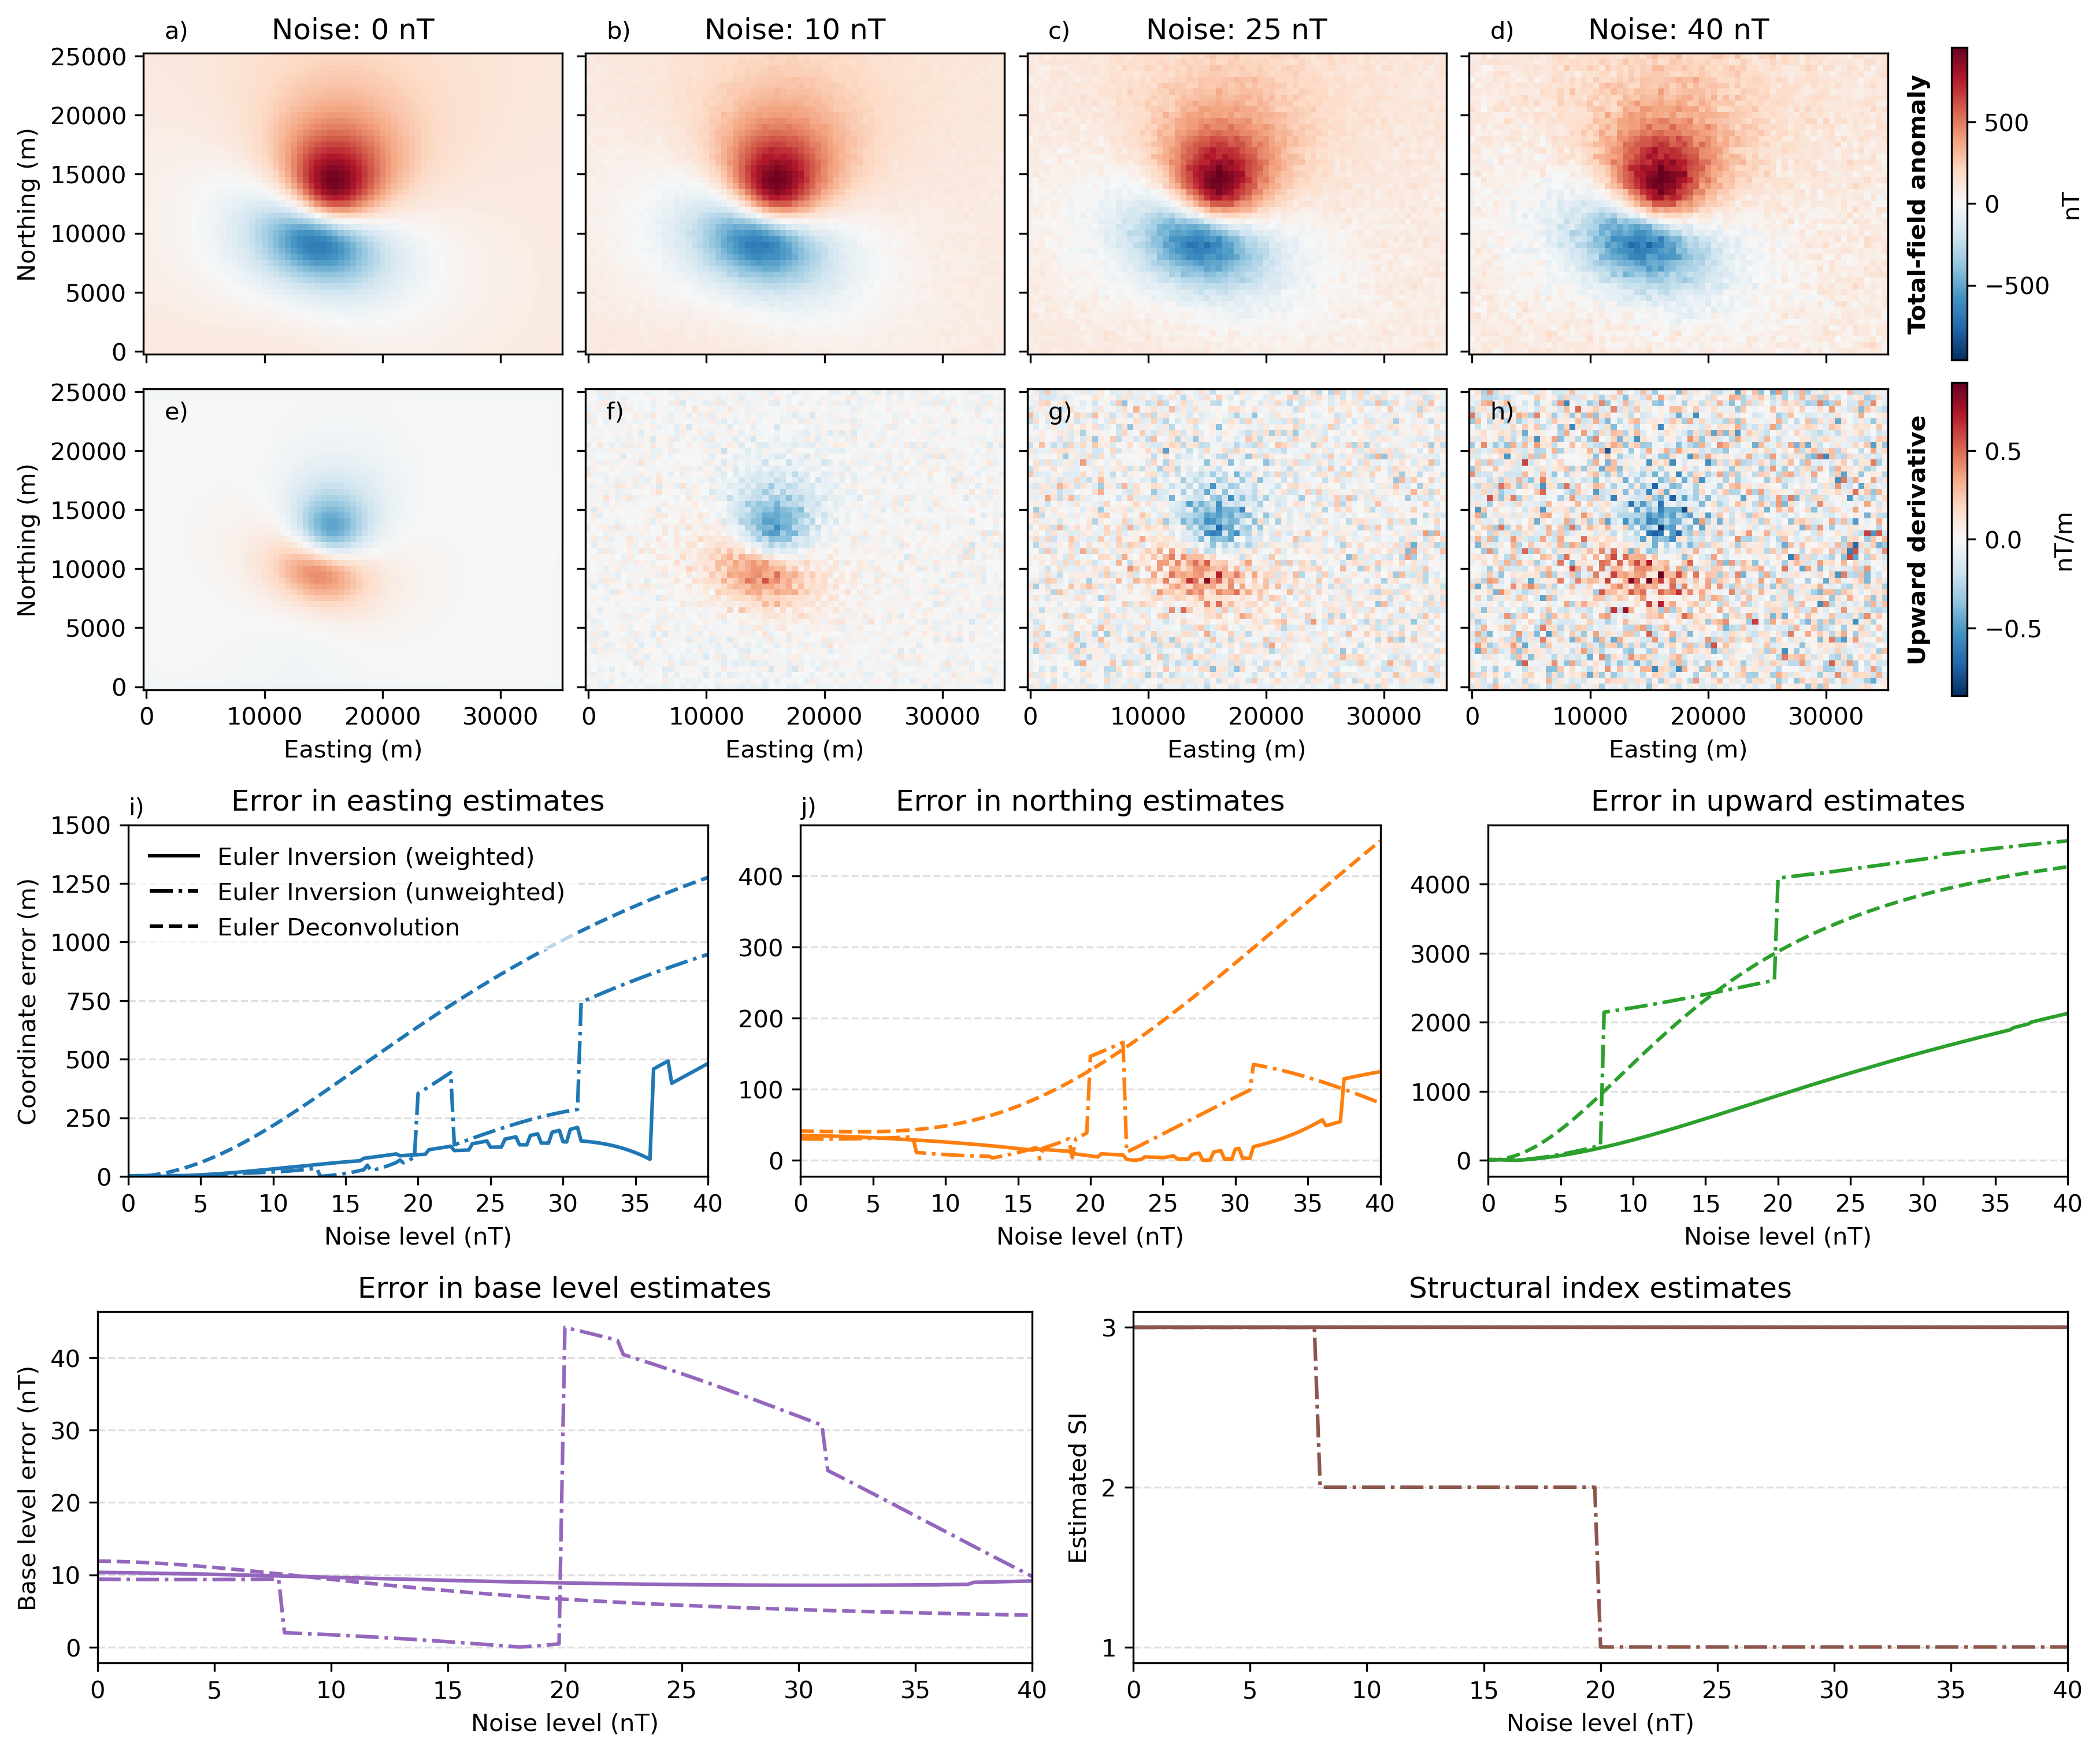
\includegraphics[width=1\linewidth]{figures/synthetic-noise-levels.png}
\caption{
  \lipsum[1]
}
\label{fig:noise}
\end{figure}

\subsection{Effect of SI on multiple sources}

\begin{figure}[tb!]
\centering
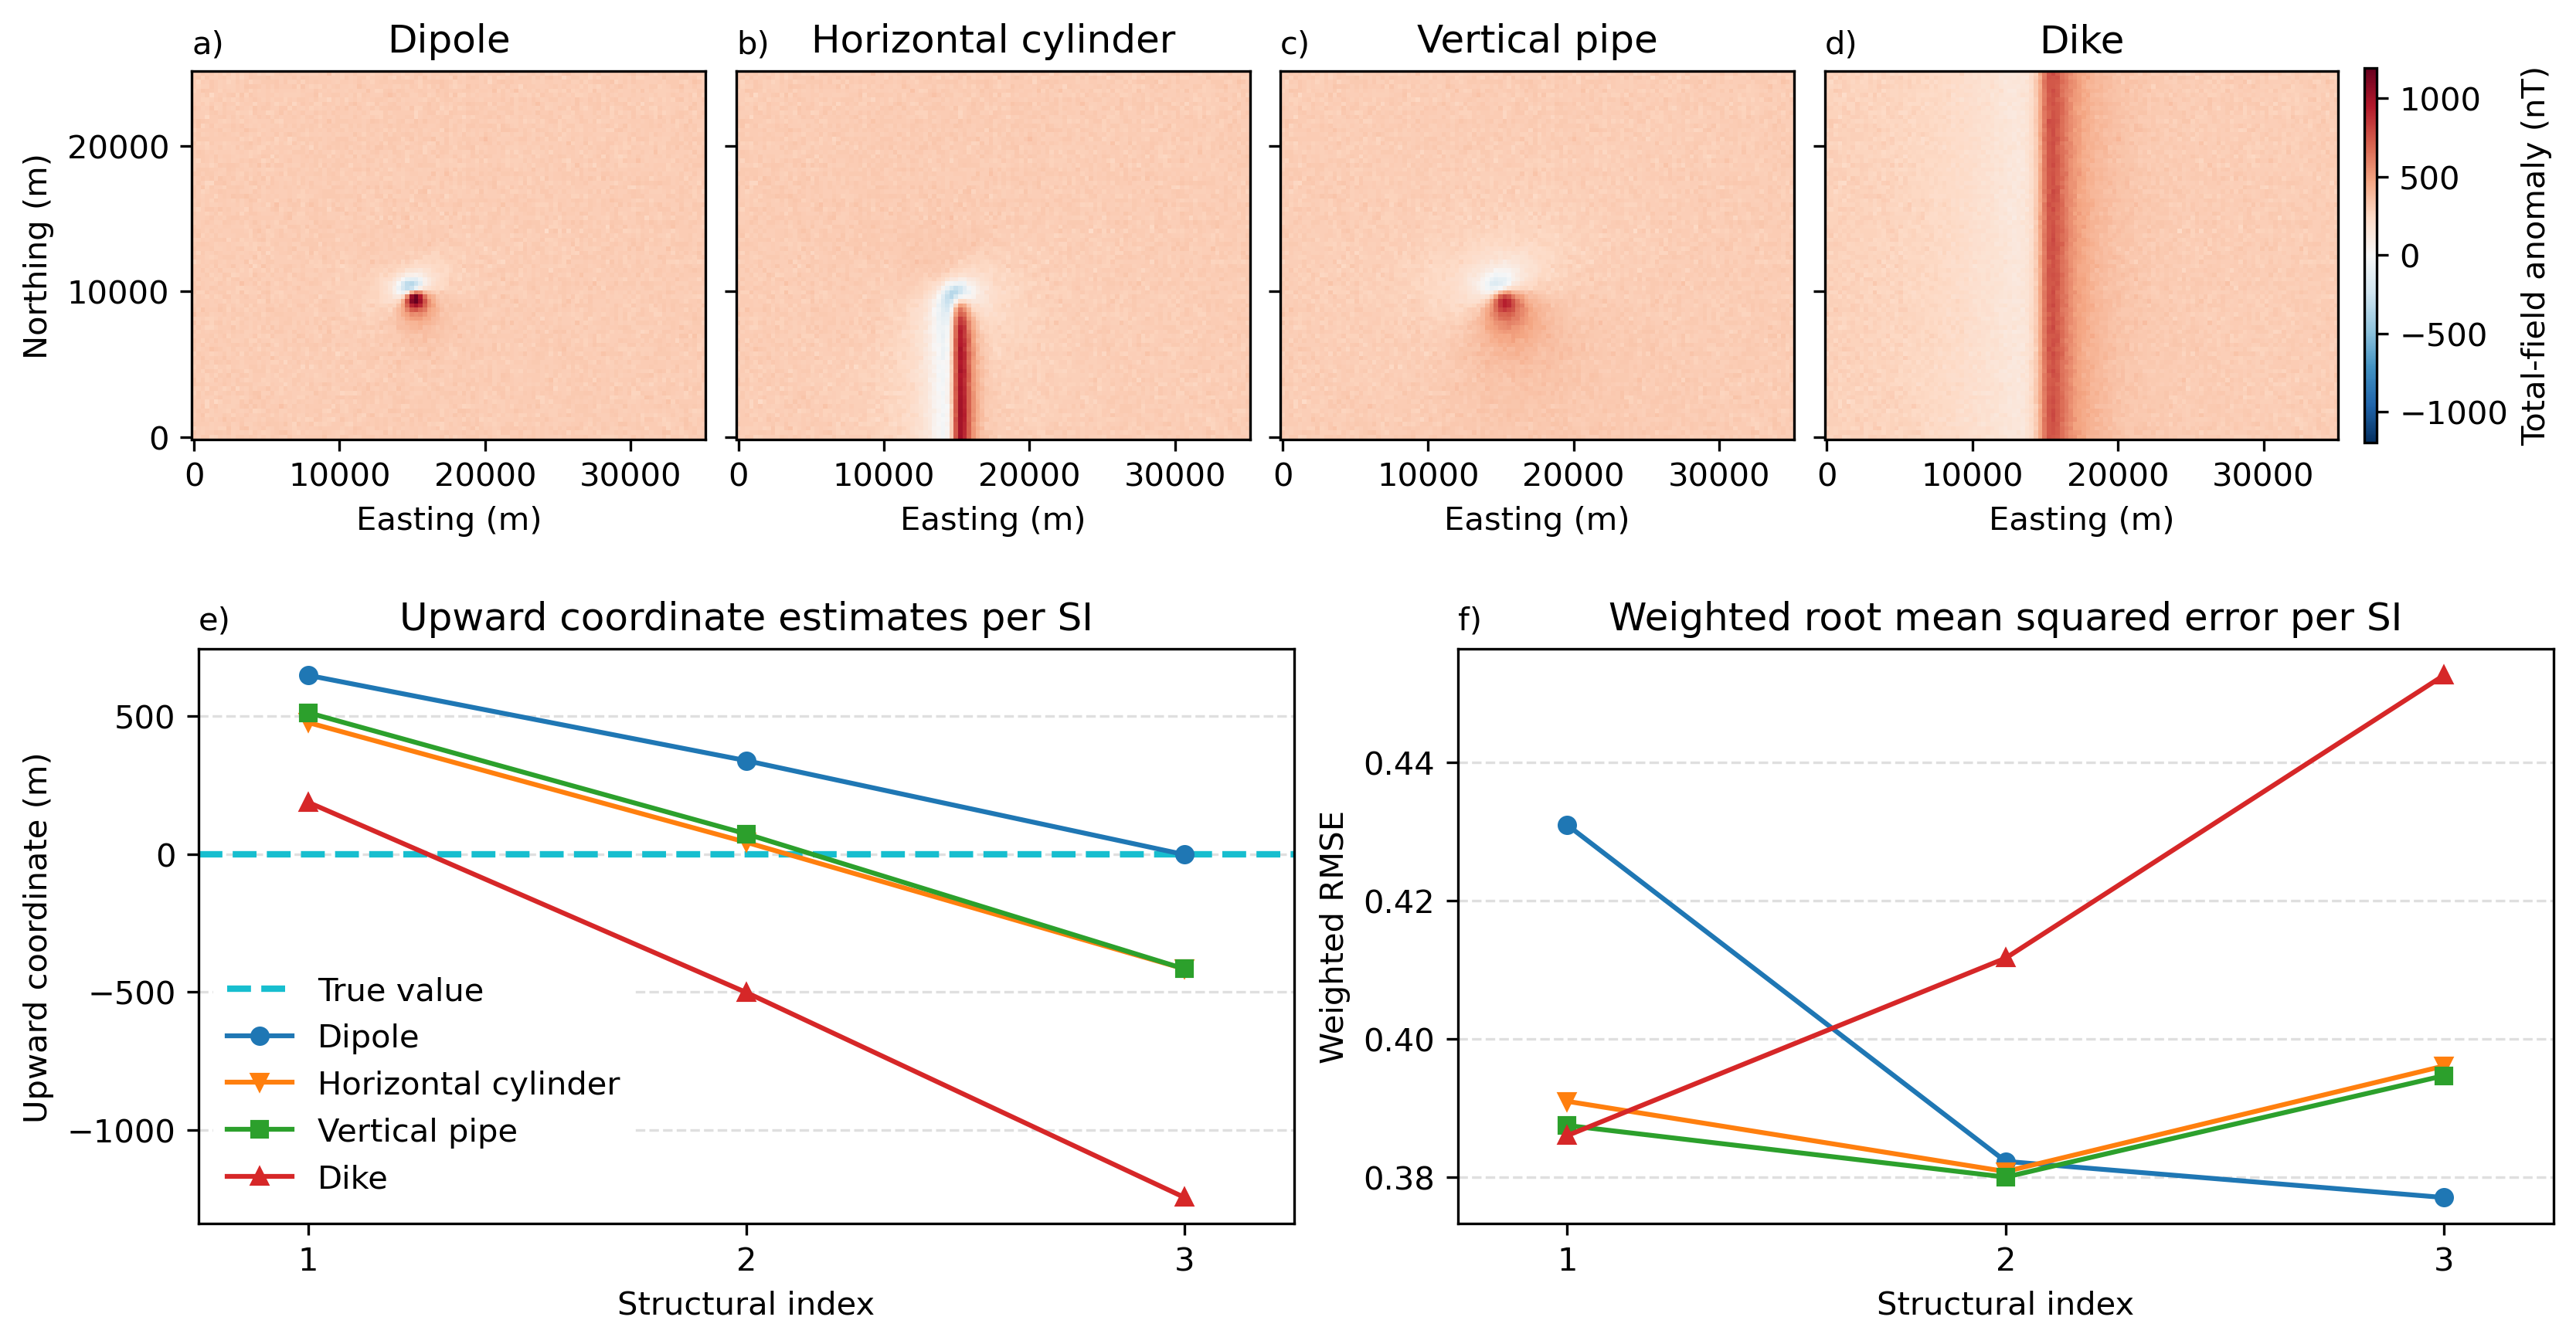
\includegraphics[width=1\linewidth]{figures/synthetic-structural-index.png}
\caption{
  \lipsum[1]
}
\label{fig:si}
\end{figure}

\subsection{Windowing procedure with multiple sources}

\begin{figure}[tb!]
\centering
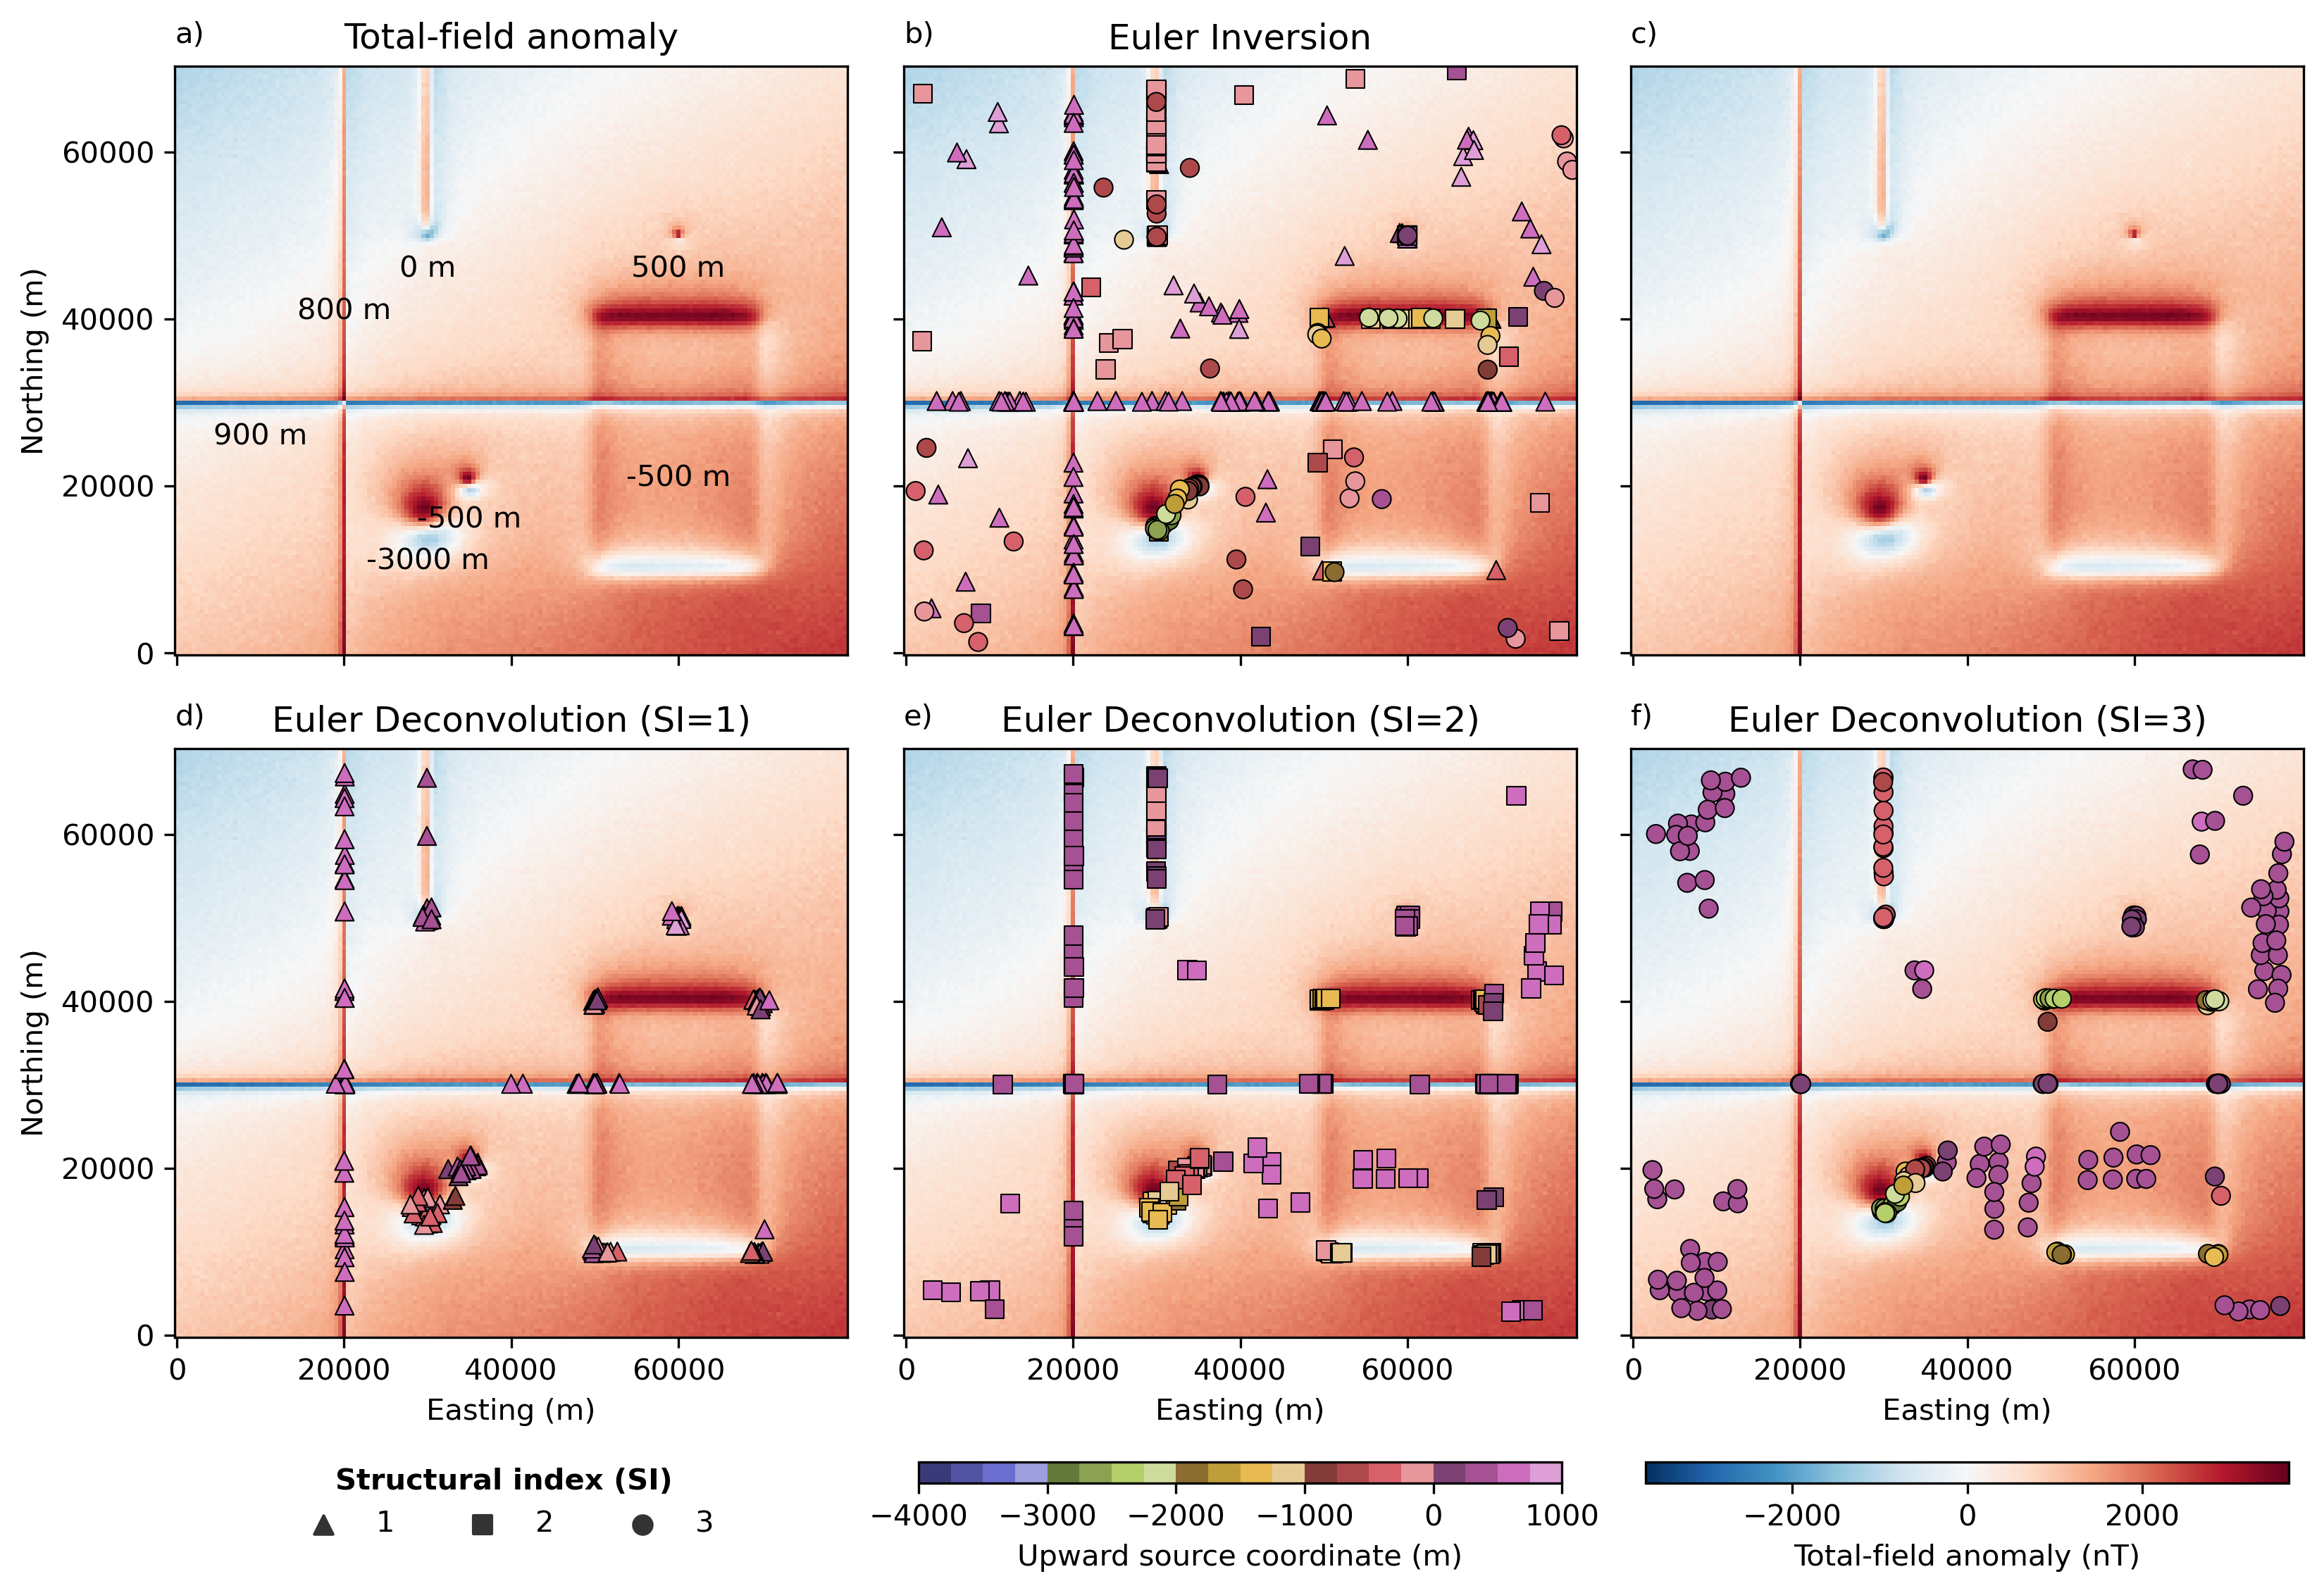
\includegraphics[width=1\linewidth]{figures/synthetic-windows.png}
\caption{
  \lipsum[1]
}
\label{fig:windows}
\end{figure}

\subsection{Aeromagnetic data from Rio de Janeiro}

%%%%%%%%%%%%%%%%%%%%%%%%%%%%%%%%%%%%%%%%%%%%%%%%%%%%%%%%%%%%%%%%%%%%%%%%%%%%%%%
\section{Conclusion}



%%%%%%%%%%%%%%%%%%%%%%%%%%%%%%%%%%%%%%%%%%%%%%%%%%%%%%%%%%%%%%%%%%%%%%%%%%%%%%%
\section{Open research}

The Python source code used to produce all results and figures presented here
is available at \url{https://github.com/\GitHubRepository} and
\url{https://doi.org/\ArchiveDOI} under the MIT open-source license.

Here we should cite all of the main software used, like Jupyter, numpy, scipy,
matplotlib, Fatiando, etc.

Cite any data sources as well.



%%%%%%%%%%%%%%%%%%%%%%%%%%%%%%%%%%%%%%%%%%%%%%%%%%%%%%%%%%%%%%%%%%%%%%%%%%%%%%%
\section{Acknowledgements}

We are indebted to the developers and maintainers of the open-source software
without which this work would not have been possible.
Acknowledge any non-author contributors to this study.
Statement about funding.

% Thank the editors and reviewers after review.
